The pruned set $\hat{\mathcal{T}}_\eta^c$ is used to define a reduced-order measurement update. To preserve the nominal chi-square calibration, the set employed at time $i$ is determined from measurements available no later than time $i-1$. The asymptotic analysis below is restricted to a subset $\mathcal S$ that remains fixed over the estimation horizon. Time-varying selection requires a separate analysis of the switched Riccati recursion.

\begin{figure}[h!]
    \centering
    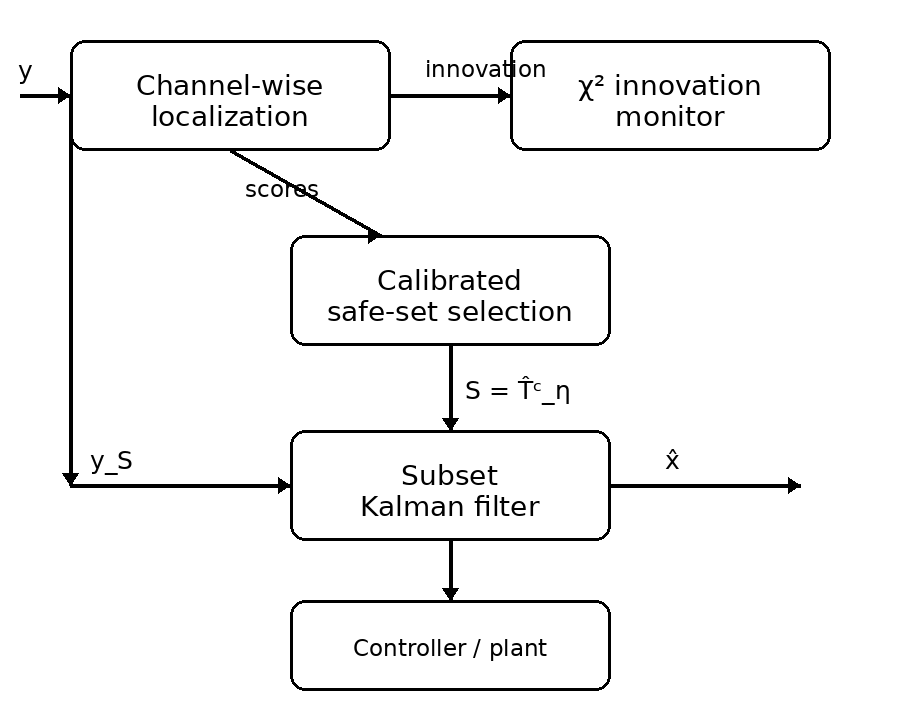
\includegraphics[width=\columnwidth]{image/resilient_L2_observer.png}
    \caption{Resilient estimation architecture. The localization and pruning stages select a sensor subset, and both the Kalman update and chi-square test are formed using that subset.}
    \label{fig:resilient_L2_observer}
\end{figure}

\subsection{Subset Kalman filter}
For a selected set $\mathcal S\subseteq\{1,\ldots,m\}$, define
\begin{equation}\label{equ:reduced_meas}
\mathbf{y}_{\mathcal S,i}=C_{\mathcal S}\mathbf{x}_i+\mathbf{v}_{\mathcal S,i}+\mathbf{e}_{\mathcal S,i}.
\end{equation}
The resilient filter applies \eqref{equ:kf_predict}--\eqref{equ:kf_Pupdate} with $(C,R)$ replaced by $(C_{\mathcal S},R_{\mathcal S})$. Its innovation statistic is
\begin{equation}\label{equ:subset_chisq}
g_i^{\mathcal S}=(\mathbf{r}_i^{\mathcal S})^\top
(S_i^{\mathcal S})^{-1}\mathbf{r}_i^{\mathcal S}.
\end{equation}
When $\mathcal S$ is selected independently of the current innovation and is attack-free, $g_i^{\mathcal S}\sim\chi_{|\mathcal S|}^2$. Hence, the threshold must be recomputed using $|\mathcal S|$ degrees of freedom; a window of $T$ independent subset innovations has $T|\mathcal S|$ degrees of freedom.

For a fixed observable subset $\mathcal S$, let $P_\infty(\mathcal S)$ denote the stabilizing filtered solution of the corresponding Riccati equation. Since $Q\succeq0$, this covariance is positive semidefinite. Additional independent measurements cannot increase the optimal filtering covariance. Therefore, for nested observable sets $\mathcal S_1\subseteq\mathcal S_2$,
\begin{equation}\label{equ:riccati_monotonicity}
P_\infty(\mathcal S_2)\preceq P_\infty(\mathcal S_1).
\end{equation}

\begin{theorem}[Conditional resilient-estimation performance]
\label{Thm:resilient_estimation_gaurentee}
Let $\mathcal S=\hat{\mathcal{T}}_\eta^c$ be fixed over the estimation horizon and suppose $\eta\le\eta_{\rm obs}$ in \eqref{equ:eta_observability}. Conditional on the event
\[
\mathcal{E}_{\mathcal S}=\{\mathcal S\cap\mathcal{T}=\varnothing\},
\]
the resilient filter is identical to the attack-free Kalman filter based on $\mathcal S$, and
\begin{equation}\label{equ:error_bound}
\lim_{i\rightarrow\infty}
\mathbb{E}\!\left[
\|\mathbf{x}_i-\hat{\mathbf{x}}_{i|i}^{\mathcal S}\|_2^2
\mid\mathcal{E}_{\mathcal S},\mathcal S
\right]
=\operatorname{tr}P_\infty(\mathcal S).
\end{equation}
Furthermore,
\begin{align}\label{equ:error_gap}
\operatorname{tr}P_\infty(\{1,\ldots,m\})
&\le\operatorname{tr}P_\infty(\mathcal S)\nonumber\\
&\le
\max_{\substack{\mathcal U\subseteq\mathcal S,\ |\mathcal U|=k_0}}
\operatorname{tr}P_\infty(\mathcal U).
\end{align}
The conditioning event satisfies
$\Pr(\mathcal{E}_{\mathcal S}\mid\mathcal G)\ge\eta$ and, consequently,
$\Pr(\mathcal{E}_{\mathcal S})\ge\eta$.
\end{theorem}
\begin{proof}
Propositions~\ref{Prop:safe_precision} and~\ref{Prop:precision_observability} give $\Pr(\mathcal{E}_{\mathcal S}\mid\mathcal G)\ge\eta$ and $|\mathcal S|\ge k_0$. Assumption~A2 then implies that $(A,C_{\mathcal S})$ is observable. On $\mathcal{E}_{\mathcal S}$, $\mathbf{e}_{\mathcal S,i}=0$ throughout the interval, so the subset-filter recursion coincides exactly with its attack-free counterpart. Standard Kalman-filter convergence gives \eqref{equ:error_bound}. The first inequality in \eqref{equ:error_gap} follows because $\mathcal S$ is contained in the full sensor set. For every $k_0$-element subset $\mathcal U\subseteq\mathcal S$, \eqref{equ:riccati_monotonicity} gives $P_\infty(\mathcal S)\preceq P_\infty(\mathcal U)$; taking the largest trace proves the second inequality.
\end{proof}

The theorem is intentionally conditional. No finite unconditional mean-square bound follows from a cleanliness probability alone because the attack magnitude on the complementary event $\mathcal{E}_{\mathcal S}^c$ may be unbounded. A trajectory-wide unconditional guarantee therefore requires either an attack-amplitude model or a robust update on the failure event.

\subsection{Quantitative performance relation}
Equations \eqref{equ:sparsity_budget}, \eqref{equ:eta_observability}, and \eqref{equ:error_gap} provide the desired quantitative relation. First, $k\le m-k_0$ is necessary for any clean observable subset to exist. Second, the calibrated probabilities determine the largest reliability level $\eta_{\rm obs}$ for which the learned selector retains at least $k_0$ sensors. Third, for every admissible $\eta$, the resulting conditional mean-square error is $\operatorname{tr}P_\infty(\mathcal S)$.

The relation also exposes a design tradeoff. Increasing $\eta$ generally reduces $l_\eta$, thereby increasing the covariance through \eqref{equ:riccati_monotonicity}; decreasing $\eta$ retains more measurements but weakens the certified probability that all retained sensors are safe. A suitable reliability level may therefore be selected by
\begin{equation}\label{equ:eta_design}
\min_{\eta\in[\eta_{\min},\eta_{\rm obs}]}
\operatorname{tr}P_\infty(\hat{\mathcal{T}}_\eta^c)
\quad
\text{subject to}\quad
\Pr(\mathcal{E}_{\hat{\mathcal{T}}_\eta^c}\mid\mathcal G)\ge\eta.
\end{equation}
Here $\eta_{\min}$ is a designer-specified reliability floor. This formulation connects localization confidence directly to the estimator covariance rather than treating observability as a binary post-processing check.
